

\tikzset{every picture/.style={line width=0.75pt}} %set default line width to 0.75pt        

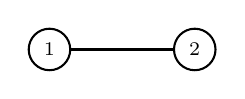
\begin{tikzpicture}[x=0.75pt,y=0.75pt,yscale=-1,xscale=1]
%uncomment if require: \path (0,162); %set diagram left start at 0, and has height of 162

%Shape: Circle [id:dp33085044400227215] 
\draw   (50,60) .. controls (50,54.48) and (54.48,50) .. (60,50) .. controls (65.52,50) and (70,54.48) .. (70,60) .. controls (70,65.52) and (65.52,70) .. (60,70) .. controls (54.48,70) and (50,65.52) .. (50,60) -- cycle ;
%Shape: Circle [id:dp45632065494671825] 
\draw   (120,60) .. controls (120,54.48) and (124.48,50) .. (130,50) .. controls (135.52,50) and (140,54.48) .. (140,60) .. controls (140,65.52) and (135.52,70) .. (130,70) .. controls (124.48,70) and (120,65.52) .. (120,60) -- cycle ;
%Straight Lines [id:da6274751888831748] 
\draw    (70,60) -- (120,60) ;

% Text Node
\draw (60,60) node  [font=\scriptsize]  {$1$};
% Text Node
\draw (130,60) node  [font=\scriptsize]  {$2$};


\end{tikzpicture}